A continuación mostramos los resultados obtenidos para el test de comparación entre factorización LU y eliminación gaussiana, los tiempos de cómputo se muestran en segundos. Se muestran los resultados de matrices de 2500x2500, 900x900 y 100x100. 


\begin{figure}[H]{}
\centering
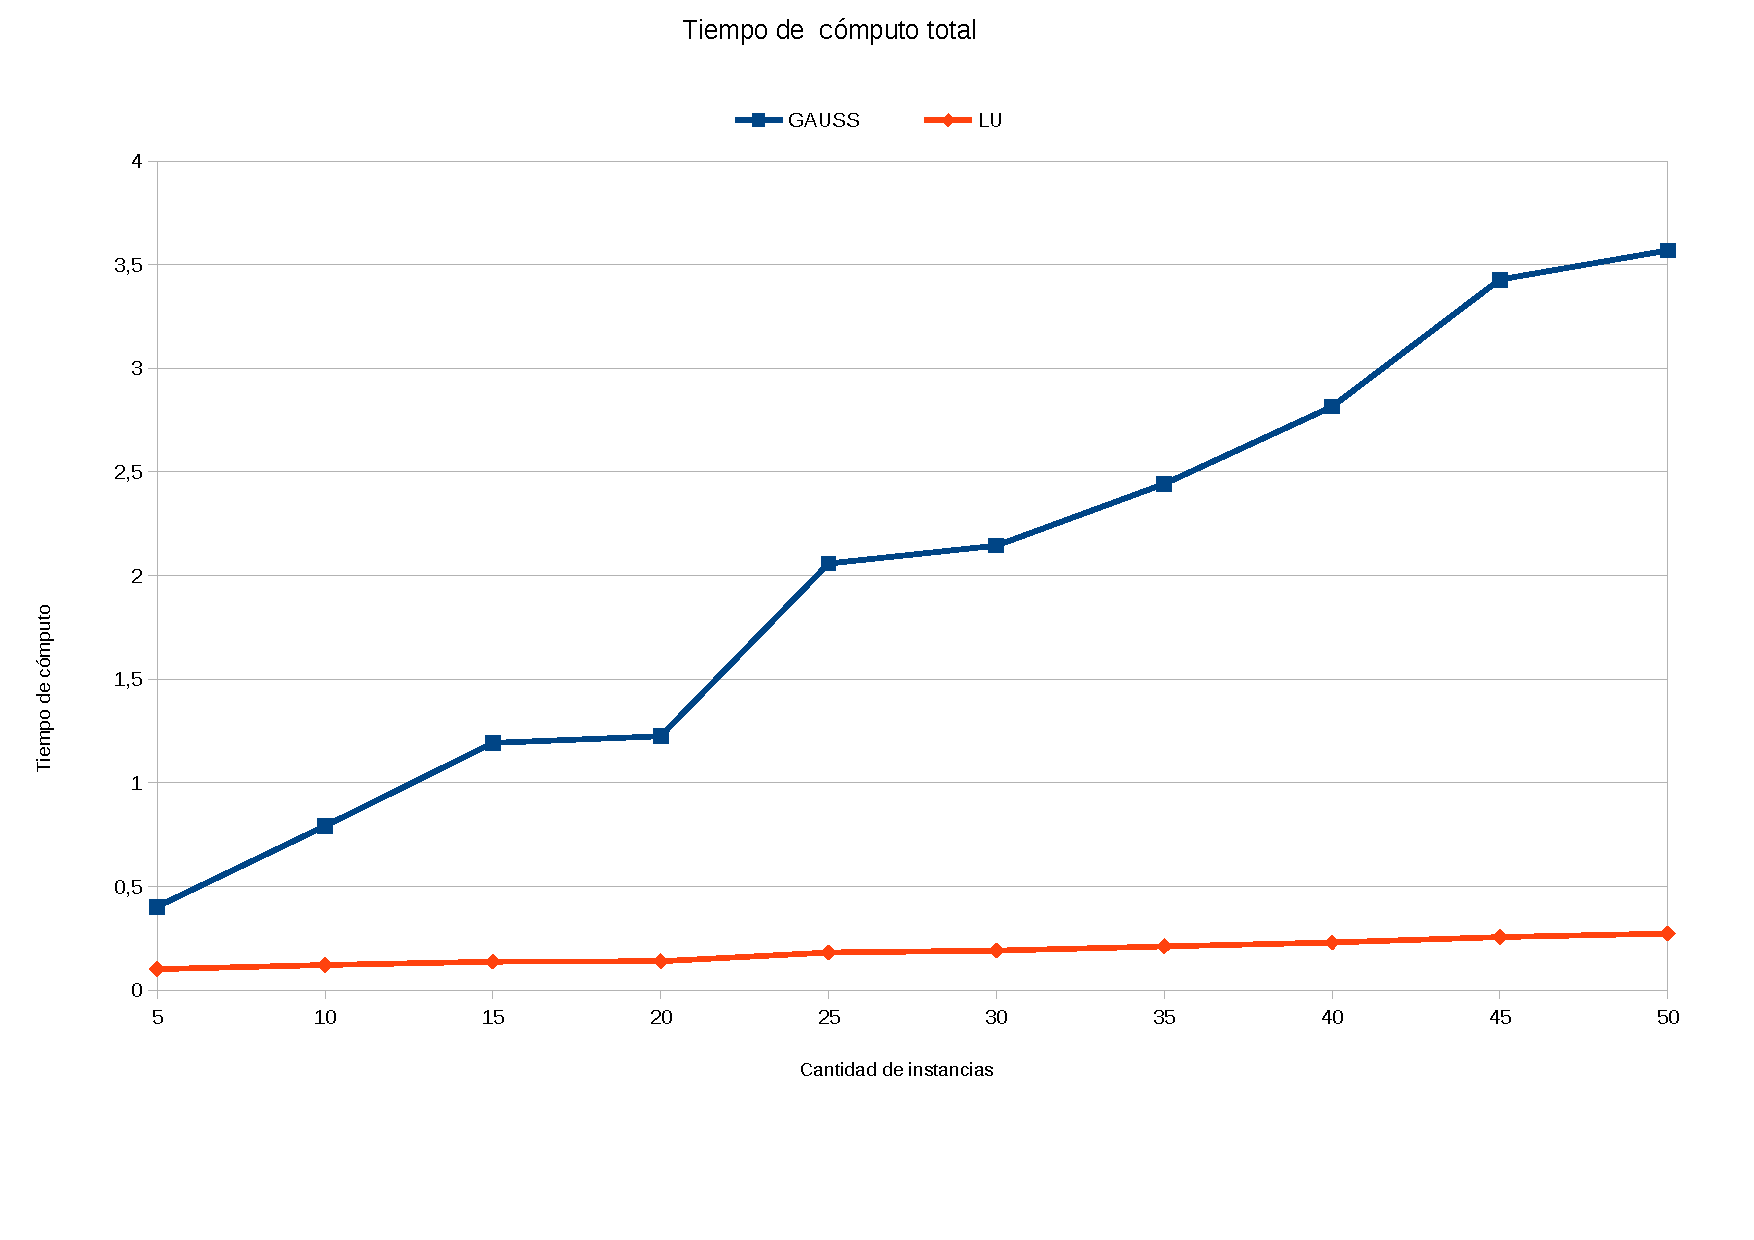
\includegraphics[scale=0.5]{graphs/gaussVsLU1.pdf}
\caption{Resultados obtenidos usando matrices de 50 ángulos y 50 radios.}
\label{gaussVsLU1}
\end{figure}

\begin{figure}[H]{}
\centering
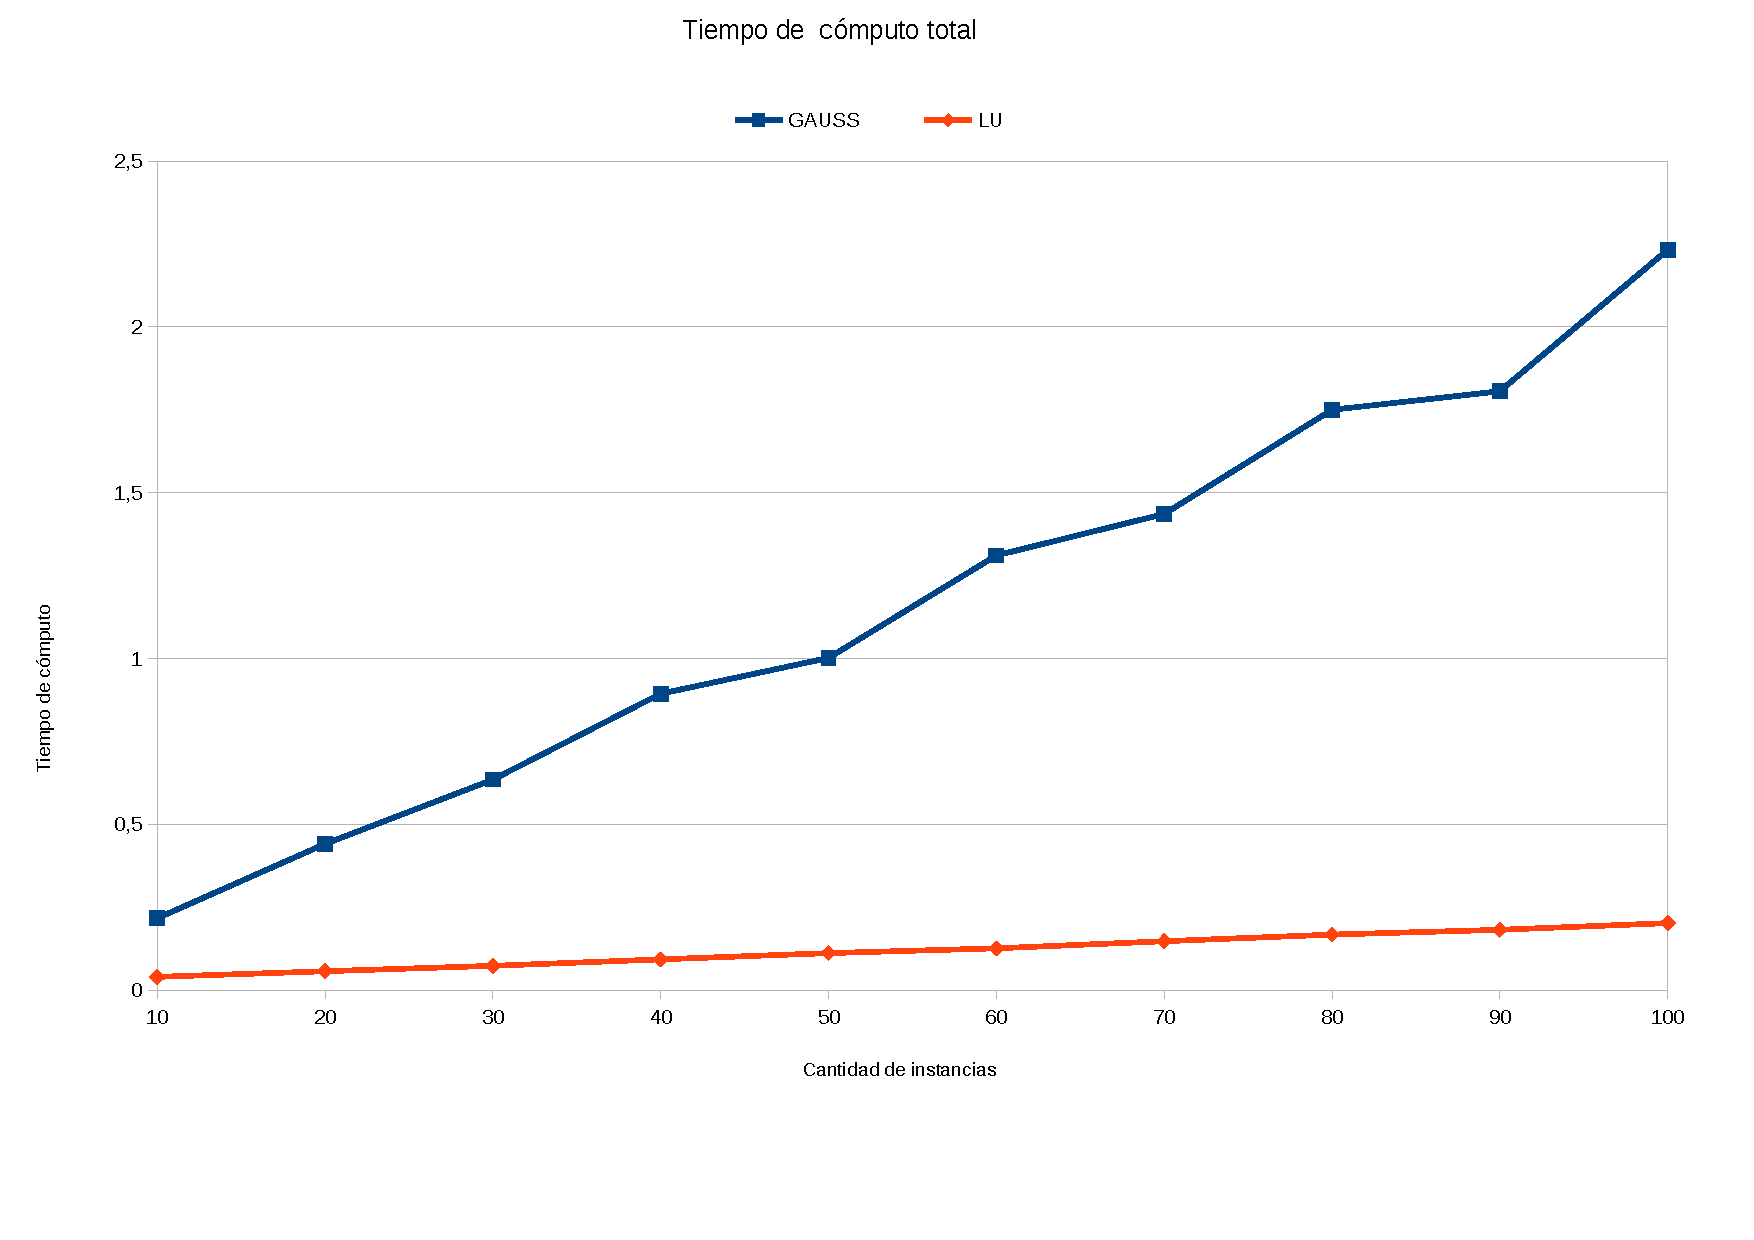
\includegraphics[scale=0.5]{graphs/gaussVsLU2.pdf}
\caption{Resultados obtenidos usando matrices de 30 ángulos y 3050 radios.}
\label{gaussVsLU2}
\end{figure}

\begin{figure}[H]{}
\centering
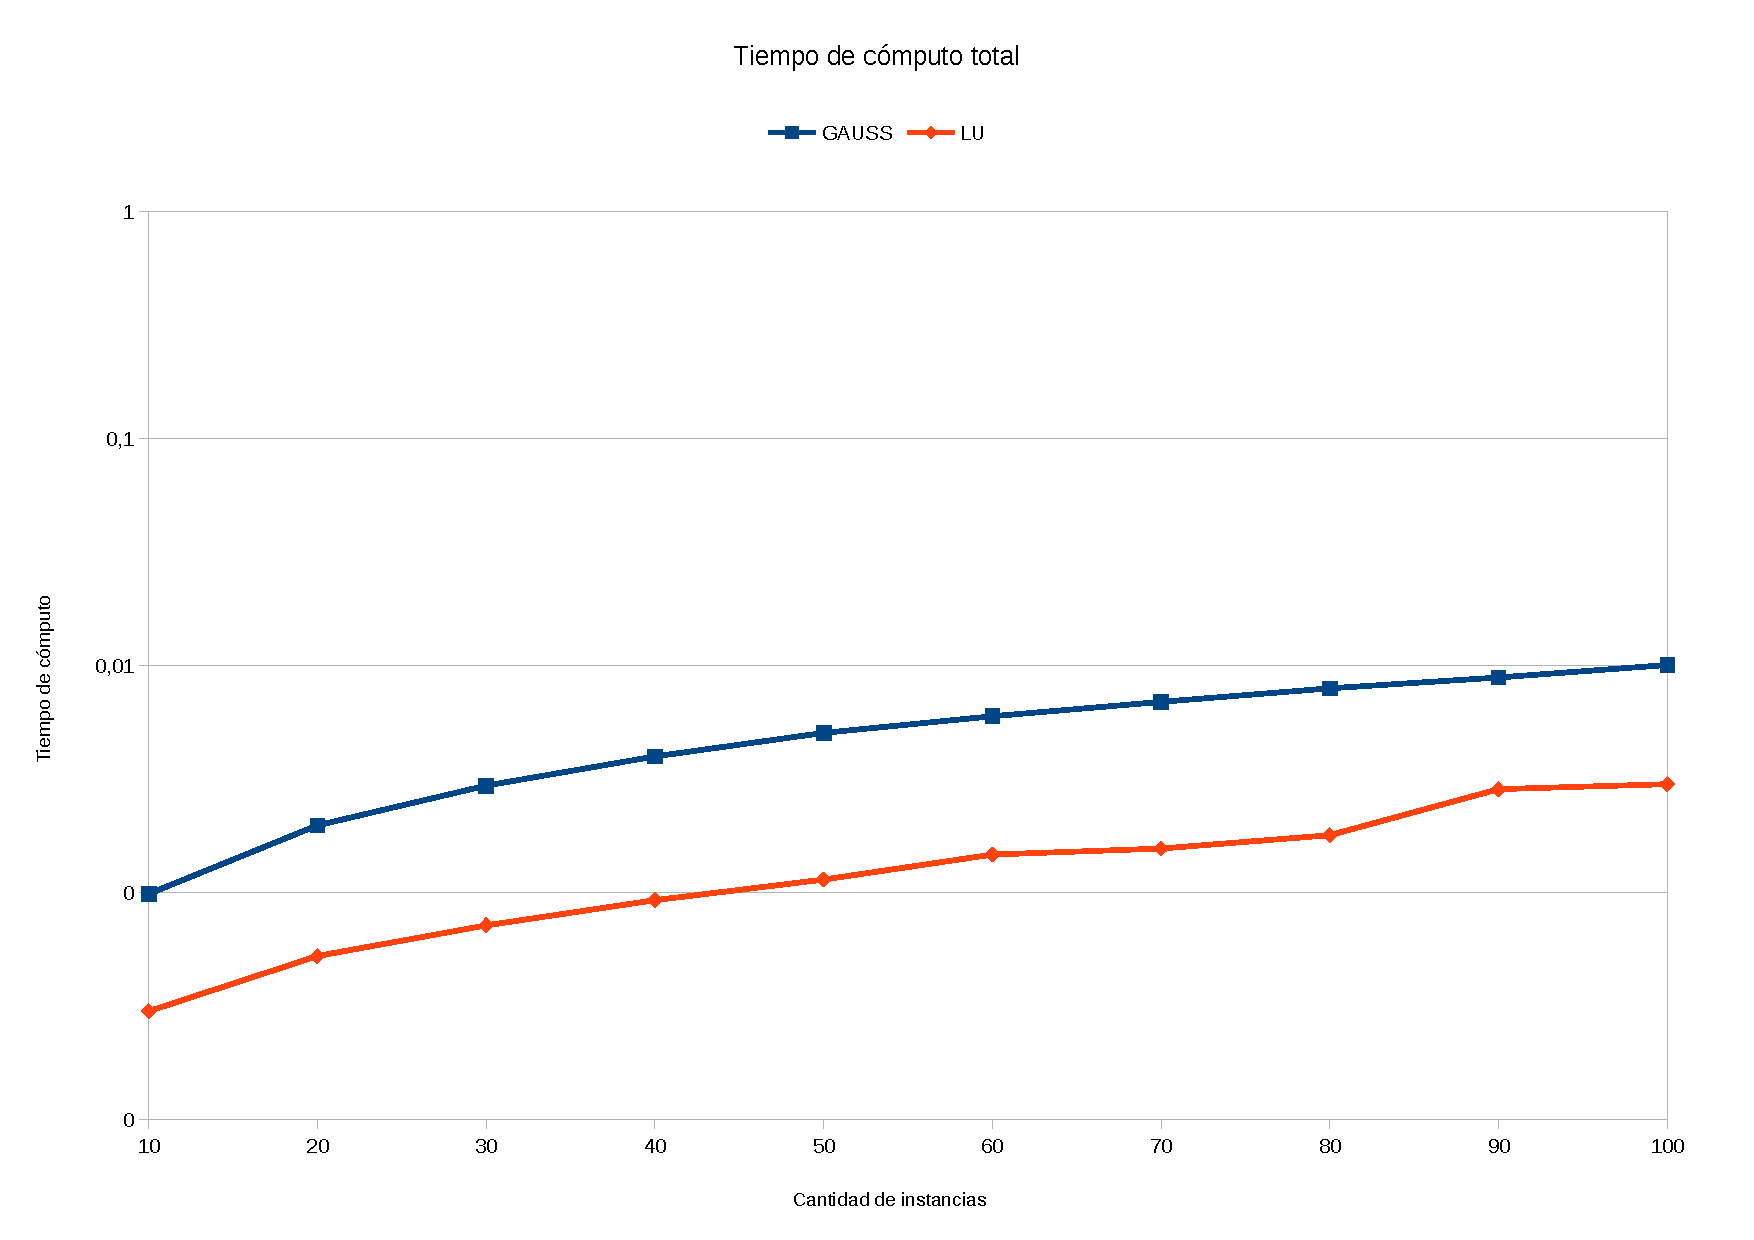
\includegraphics[scale=0.5]{graphs/gaussVsLU3.pdf}
\caption{Resultados obtenidos usando matrices de 10 ángulos y 10 radios.}
\label{gaussVsLU3}


\end{figure}
